\documentclass[a4paper,12pt]{article}
\usepackage[utf8]{inputenc}
\usepackage[T2A]{fontenc}
\usepackage[russian,english]{babel}
\usepackage[pdftex]{graphics}
\DeclareGraphicsExtensions{.pdf,.png,.jpg}
\graphicspath{{pictures/}}
\begin{document}
\begin{center}
Санкт-Петербургский государственный политехнический университет
\\Кафедра компьютерных систем и программных технологий
\end{center}
\vspace*{10em plus .6em minus .5em}

\begin{center}
{\LARGEТелекоммуникационные технологии
\\Лабораторная работа №3
\\Линейная фильтрация}
\end{center}

\vspace*{5em plus .6em minus .5em}
\begin{flushright}
Выполнил:\\студент гр.33501/4\\Корсков Алексей\\Проверила:\\Богач Н.В.
\end{flushright}

\vspace*{15em plus .6em minus .5em}
\begin{center}
{\smallСанкт-Петербург
\\2018}
\end{center}
\pagestyle{empty}
\newpage
\pagestyle{plain}
{\bfseriesЦель}

Изучить воздействие ФНЧ на тестовый сигнал с шумом.

{\bfseriesПостановка задачи}

Сгенерировать гармонический сигнал с шумом и синтезировать ФНЧ. Получить сигнал во временной и частотной областях до и после фильтрации. Сделать выводы о воздействии ФНЧ на спектр сигнала.

{\bfseriesТеоретическое обоснование}

Фильтр в электронике — устройство для выделения желательных компонентов спектра электрического сигнала и/или подавления нежелательных.

Фильтры делятся на {\bfseriesаналоговые} и {\bfseriesцифровые}. Аналоговые  имеют дело с аналоговыми или непрерывными сигналами. В отличие от них цифровые имеют дело с дискретными сигналами.

На {\bfseriesпассивные} и {\bfseriesактивные}. Пассивный фильтр — электронный фильтр, состоящий только из пассивных компонентов, таких как, к примеру, конденсаторы и резисторы. Активный фильтр — один из видов аналоговых электронных фильтров, в котором присутствует один или несколько активных компонентов, к примеру, транзистор или операционный усилитель.

На {\bfseriesлинейные} и {\bfseriesнелинейные}. Линейный фильтр — динамическая система, применяющая некий линейный оператор ко входному сигналу для выделения или подавления определённых частот сигнала и других функций по обработке входного сигнала. Нелинейный фильтр — устройство для обработки сигналов, выход которого не является линейным оператором от входного сигнала.

На {\bfseriesрекурсивные} и {\bfseriesнерикурсивные}. Рекурсивный фильтр (БИХ-фильтр) - линейный электронный фильтр, использующий один или более своих выходов в качестве входа, то есть образующий обратную связь. Такие фильтры могут быть как аналоговыми, так и цифровыми. Нерекурсивный фильтр (КИХ-фильтр) -  один из видов линейных цифровых фильтров, характерной особенностью которого является ограниченность по времени его импульсной характеристики (с какого-то момента времени она становится точно равной нулю). Такой фильтр называют ещё нерекурсивным из-за отсутствия обратной связи.

По тому, какие частоты фильтром пропускаются (задерживаются), фильтры подразделяются на
\begin{itemize}
	\item фильтры нижних частот -  электронный или любой другой фильтр, эффективно пропускающий частотный спектр сигнала ниже некоторой частоты (частоты среза) и подавляющий частоты сигнала выше этой частоты.;
	\item фильтры верхних частот -  электронный или любой другой фильтр, пропускающий высокие частоты входного сигнала, при этом подавляя частоты сигнала ниже частоты среза.;
	\item полосно-пропускающие фильтры -  фильтр, который пропускает частоты, находящиеся в некоторой полосе частот. Полосовой фильтр — линейная система и может быть представлен в виде последовательности, состоящей из фильтра нижних частот и фильтра верхних частот.;
	\item полосно-задерживающие фильтры -  электронный или любой другой фильтр, не пропускающий колебания некоторой определённой полосы частот, и пропускающий колебания с частотами, выходящими за пределы этой полосы.;
	\item фазовые фильтры - электронный или любой другой фильтр, пропускающий все частоты сигнала с равным усилением, однако изменяющий фазу сигнала..
\end{itemize}
\newpage

{\LargeХод работы}
\begin{enumerate}
{\itemСгенерируем гармонический сигнал
\center{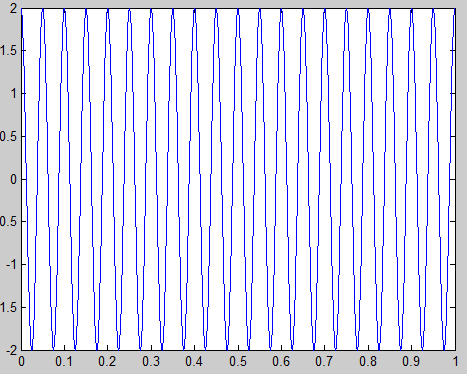
\includegraphics{./pictures/Signal.png} \\ Рис.1 Сигнал}
\center{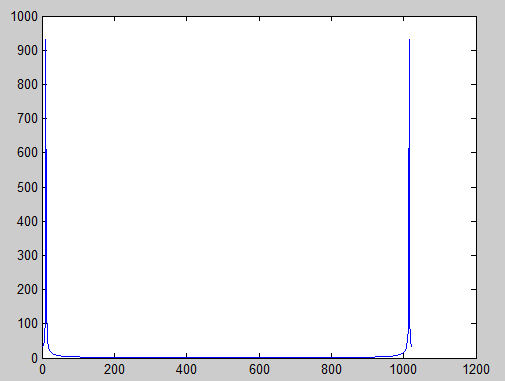
\includegraphics{./pictures/SpecSignal.png} \\ Рис.2 Спектр сигнала}
\\}

{\itemДобавим к нему шум
\center{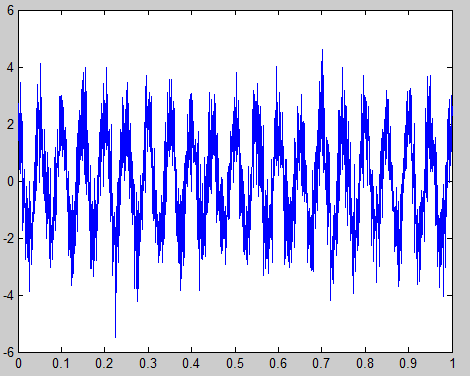
\includegraphics{./pictures/Noise.png} \\ Рис.3 Зашумленный сигнал}
\center{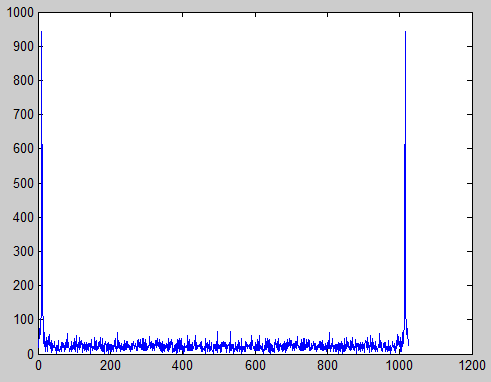
\includegraphics{./pictures/SpecNoise.png} \\ Рис.4 Спектр зашумленного сигнала}
\\}

{\itemВыполним фильтрацию сигнала
\center{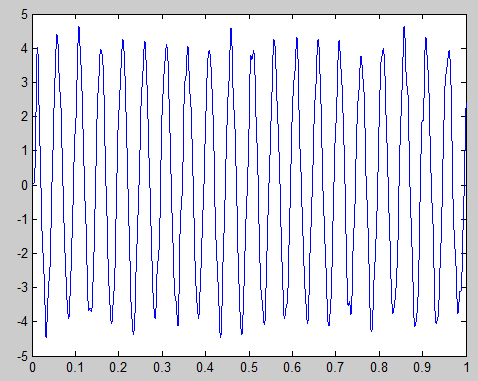
\includegraphics{./pictures/SignalNoise.png} \\ Рис.5 Сигнал после фильтрации}
\center{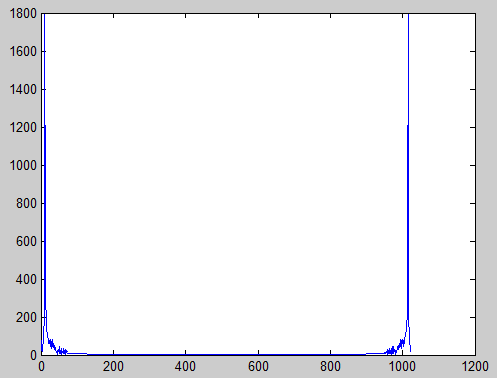
\includegraphics{./pictures/SpecSignalNoise.png} \\ Рис.6 Спектр сигнала после фильтрации}
\\}

{\itemСгенерируем гармонический сигнал в Simulink
\center{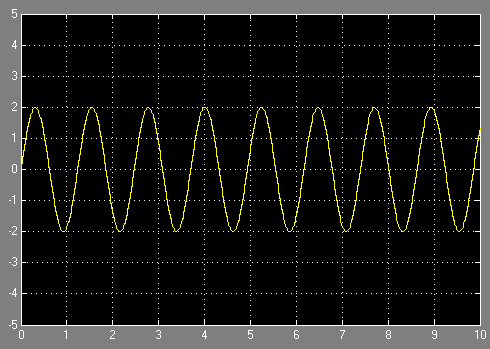
\includegraphics{./pictures/SimulSignal.png} \\ Рис.7 Сигнал}
\center{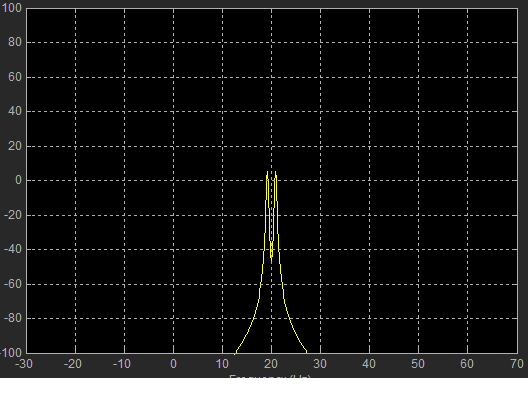
\includegraphics{./pictures/SimulSpecSignal.png} \\ Рис.8 Спектр сигнала}
\\}

{\itemДобавим к нему шум
\center{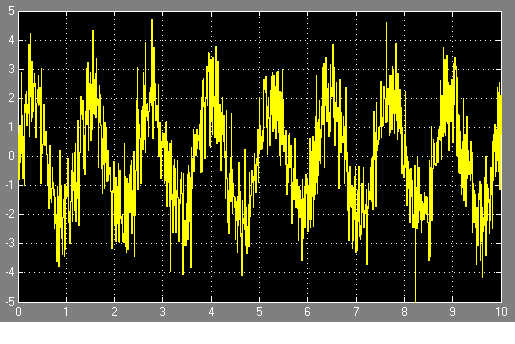
\includegraphics{./pictures/SimulNoise.png} \\ Рис.9 Зашумленный сигнал}
\center{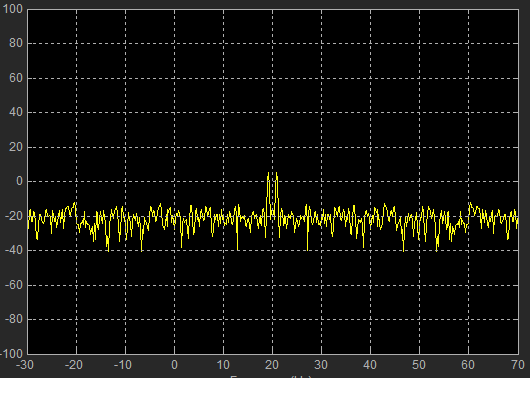
\includegraphics{./pictures/SimulSpecNoise.png} \\ Рис.10 Спектр зашумленного сигнала}
\\}

{\itemВыполним фильтрацию сигнала
\center{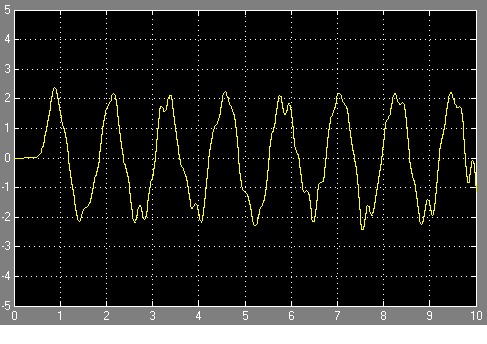
\includegraphics{./pictures/SimulSignalNoise.png} \\ Рис.11 Сигнал после фильтрации}
\center{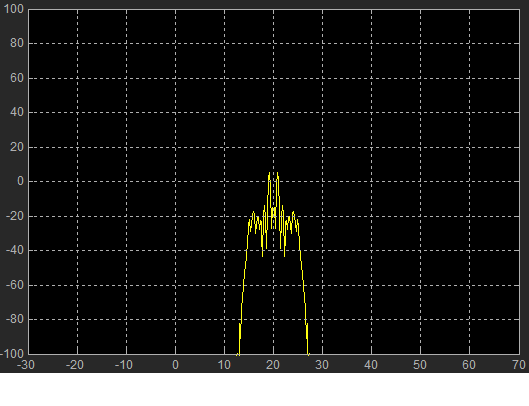
\includegraphics{./pictures/SimulSpecSignalNoise.png} \\ Рис.12 Спектр сигнала после фильтрации}
\\}

{\bfseries\LARGEВывод}

В ходе выполнения лабораторной работы мы познакомились с ФНЧ и применили его на тестовый сигнал с шумом. Был создан сигнал, зашумлен и отфильтрован как в Matlab, так и в Simulink. Видно, что действительно ФНЧ отфильтровал сигнал, но он не полностью совпадает с исходным. Это объясняется тем, что часть шума имеет низкие частоты, которые фильтр не может подавить и именно этот шум искажает наш сигнал.

\end{enumerate}
\end{document}
